\documentclass[12pt, twoside]{article}
\usepackage{jmlda}
\newcommand{\hdir}{.}

\renewcommand{\baselinestretch} {1.35}
\usepackage{xcolor}

\usepackage[english, russian]{babel}
\usepackage[utf8]{inputenc}

% The package for images
\usepackage{graphics}
\usepackage{graphicx}
\usepackage{caption}
\usepackage{subfig}
\graphicspath{{phase/}}
\DeclareGraphicsExtensions{.pdf,.png,.jpg}

% Доп пакеты
\usepackage[usenames]{color}
\usepackage{colortbl}

% The package for text in angle
\usepackage{booktabs}

% The package for Gothic letters
\usepackage{amssymb}

% The algorithmicx package for pseudocode
\usepackage{algorithm} 
\usepackage{algorithmic} 


\newcommand{\N}{\mathbb{N}}
\newcommand{\Z}{\mathbb{Z}}
%https://www.overleaf.com/project/6034bac8be0902011ffeee39
\theoremstyle{definition}

\newenvironment{theorem}[2][Теорема]{\begin{trivlist}
\item[\hskip \labelsep {\bfseries #1}\hskip \labelsep {\bfseries #2.}]}{\end{trivlist}}
\newenvironment{lemma}[2][Lemma]{\begin{trivlist}
\item[\hskip \labelsep {\bfseries #1}\hskip \labelsep {\bfseries #2.}]}{\end{trivlist}}
\newenvironment{exercise}[2][Задача]{\begin{trivlist}
\item[\hskip \labelsep {\bfseries #1}\hskip \labelsep {\bfseries #2.}]}{\end{trivlist}}
\newenvironment{reflection}[2][Reflection]{\begin{trivlist}
\item[\hskip \labelsep {\bfseries #1}\hskip \labelsep {\bfseries #2.}]}{\end{trivlist}}
\newenvironment{proposition}[2][Proposition]{\begin{trivlist}
\item[\hskip \labelsep {\bfseries #1}\hskip \labelsep {\bfseries #2.}]}{\end{trivlist}}
\newenvironment{corollary}[2][Corollary]{\begin{trivlist}
\item[\hskip \labelsep {\bfseries #1}\hskip \labelsep {\bfseries #2.}]}{\end{trivlist}}


\def\eps{\varepsilon}
\def\T{{\cal T}}
\def\H{{\cal H}}
\def\K{{\cal K}}
\def\L{{\cal L}}
\def\F{{\cal F}}
\def\Q{{\cal Q}}
\def\N{{\cal N}}
\def\p{{\cal P}}
\def\np{{\cal NP}}
\def\A{{\cal A}}
\def\B{{\cal B}}
\def\D{{\cal D}}
\def\BB{{\cal B}^* }
\def\DD{{\cal D}^* }
\def\TT{\tilde{\cal T}}
\def\f{\tilde f}
\def\ind{\mathop{\rm index}}
\def\St{\mathop{\rm St}}
\let\bd\partial
\def\V{\ensuremath{{\cal V}}}
\def\SS{{\mathbb S}}
\def\RR{\mathbb R}
\def\QQ{\mathbb Q}
\def\PP{\mathbb P}
\def\AA{\mathbb A}
\def\R{\cal R}
\def\NN{\mathbb N}
\def\CC{\mathbb C}
\def\ZZ{\mathbb Z}
\def\s{\sigma}
\def\S{\Sigma }
\def\ss{\Sigma^* }
\def\ra{\rightarrow}
\def\da{\downarrow}
\def\Ra{\Rightarrow}
\def\t{\theta}

\begin{document}

Данная работа посвящена задаче восстановления фазы квазипериодического сигнала движения человека. То есть сигнала, имеющего повторяющиеся значения в данных, но не обладающего явной периодичностью. Данные собраны с трехосевого акселерометра
    \begin{equation}\label{ts}
        \{ s_i \}_{i = 1}^{N},
        \quad
        s_i = \sqrt{a_{ix}^2 + a_{iy}^2 + a_{iz}^2}
        \quad
        s_i \in \RR^1.
    \end{equation}
    
В работе предлагается алгоритм определения фазы, который основан на представлении исходного временного ряда в фазовом пространстве. Переход в фазовое пространство осуществляется с помощью построения ганкелевой матрицы
    \[ \mathbf{H} = \begin{bmatrix}
                        s_1 & \dots & s_k \\
                        s_2 & \dots & s_{k+1} \\
                        \hdotsfor{3} \\
                        s_{n} & \dots & s_{N}
                    \end{bmatrix} = 
                    \begin{bmatrix}
                        \mathbf{s}_1,
                        \mathbf{s}_2, 
                        \dots,
                        \mathbf{s}_k
                    \end{bmatrix}, \quad k = N - n + 1 \]
где~$n$ -- ширина окна.

Размерность исходного фазового пространства избыточна.
Требуется построить модель, аппроксимирующую фазовую траекторию с помощью минимального числа главных компонент.
С помощью аппроксимирующей модели определить оптимальную размерность фазового подпространства $ \mathbf{X} $.

В качестве аппроксимирующей модели математического ожидания фазовой траектории $\Expect(\mathbf{x}|\varphi):~\varphi~\rightarrow~\mathbf{x}$ предлагается регрессии Надарая-Ватсона. Аналогично предлагается ввести и модель дисперсии $\Variance(\mathbf{x}|\varphi)$.

В найденном пространстве оптимальной размерности строится алгоритм восстановления фазы временного ряда.

Оптимальная размерность пространства - это размерность пространства, в которой выполняется критерий отсутствия самопересечений.

Самопересечением фазовой траектории - это наличие близких по дисперсии точек в фазовом пространстве при существенно разных значениях фаз.
Значения фазы называются существенно разными, если их разность превосходит $\frac{\pi}{2}$.

Основная идея алгоритма базируется на трех предположениях:
\begin{enumerate}
    \item Во временном ряду~\eqref{ts} присутствует только один фиксированный класс движений; 
    
    \item Более поздним по времени точкам соответствует большая фаза.  
    Если $t > t'$, то $\varphi_t > \varphi_{t'}$ для~$t,\, t' \in [0,+\infty)$;
    
    \item Фазы соседних точек близки. Если $\| \mathbf{x} - \mathbf{x}' \|_2 < \eps$ ($\eps$ -- гиперпараметр), то $\| \varphi - \varphi' \| < \delta$ для некоторого $\delta$.
\end{enumerate}

Для выбора значения фазы введем функцию потерь из трех слагаемых.

Первая часть функции потерь $L_1$ опирается на второе предположение. Она штрафует за уменьшение значения фазы.
Вторая часть функции потерь опирается на третье предположение.
Она учитывает увеличение суммарной разницы в значениях фазы для соседствующих точек фазовом пространстве.
Третья часть учитывает расстояние от текущей точки до точек аппроксимирующей модели.
Таким образом, задача нахождения фазы для текущей точки $\mathbf{x}_i$ имеет вид
\begin{equation} 
\widehat{\varphi}_i = \arg\min_{\varphi \in \Phi_i} \lambda_1\cdot L_1(\varphi) + \lambda_2 \cdot L_2(\varphi) + \lambda_3 \cdot L_3(\varphi).
\label{eq:argminL} 
\end{equation}
где $\lambda_1, \lambda_2, \lambda_3$ - весовые коэффициенты такие, что $\sum_{i=1}^{3} \lambda_i = 1$.

В таблице \ref{tbl:table_of_figures} представлены результаты работы алгоритма для случаев ходьбы и велопрогулки. В данной работе также исследуются другие классы движения человека, пробуются различные варианты функции потерь, проводится сравнение с другими существующими методами.

\begin{table}
    \centering
        \begin{tabular}{p{0.5cm}p{4cm}p{4cm}p{5cm}}
            \toprule
              & Временной ряд & Фазовая траектория в 3D & Результат работы\\
            \midrule
            \rotatebox{90}{ \text{Ходьба} }
            & 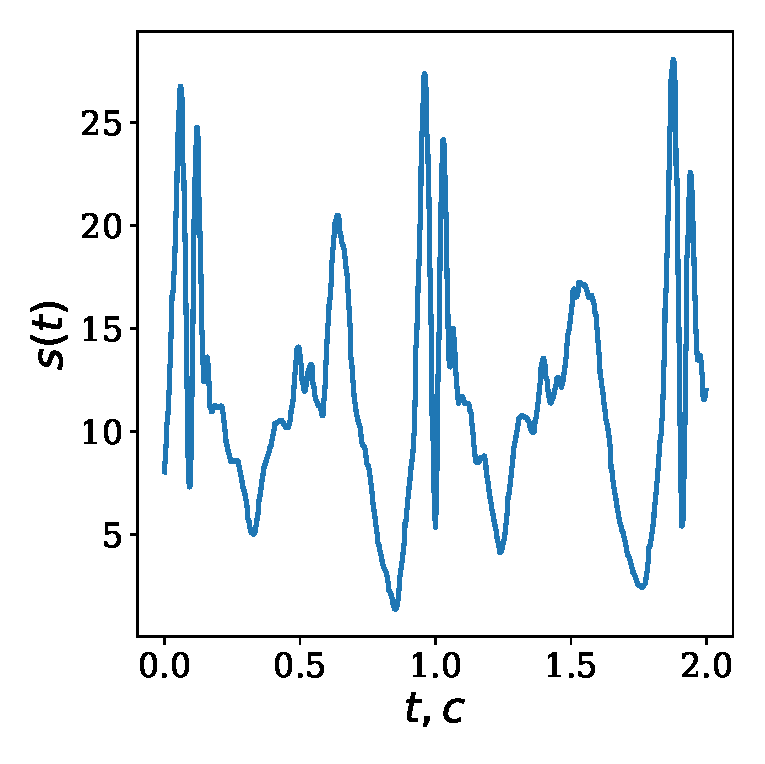
\includegraphics[scale=0.25]{./images/walk_example.eps}
            & 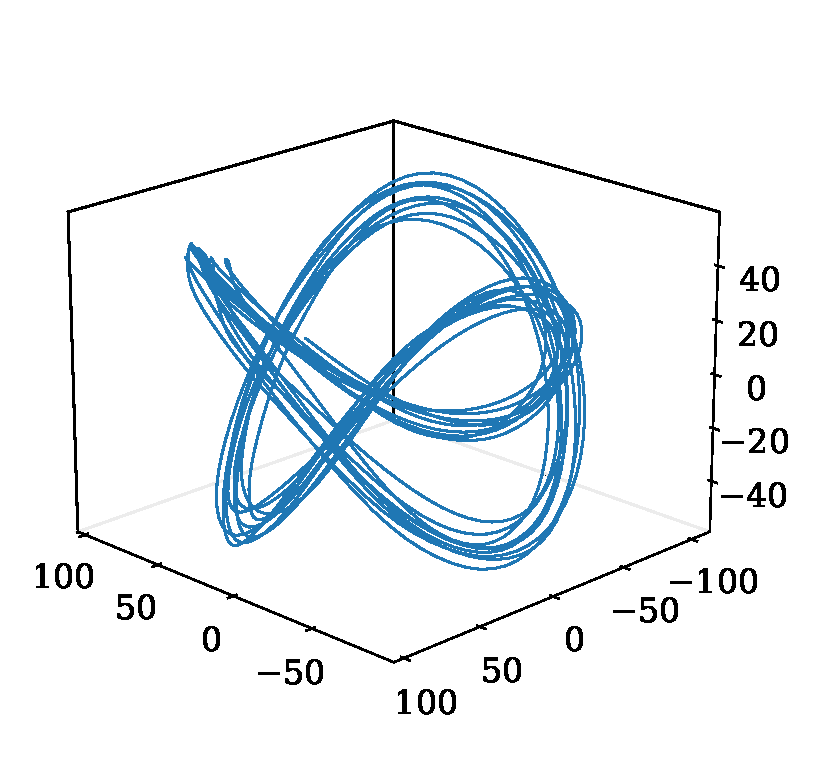
\includegraphics[scale=0.3]{./images/walk_trajectory.eps}
            & 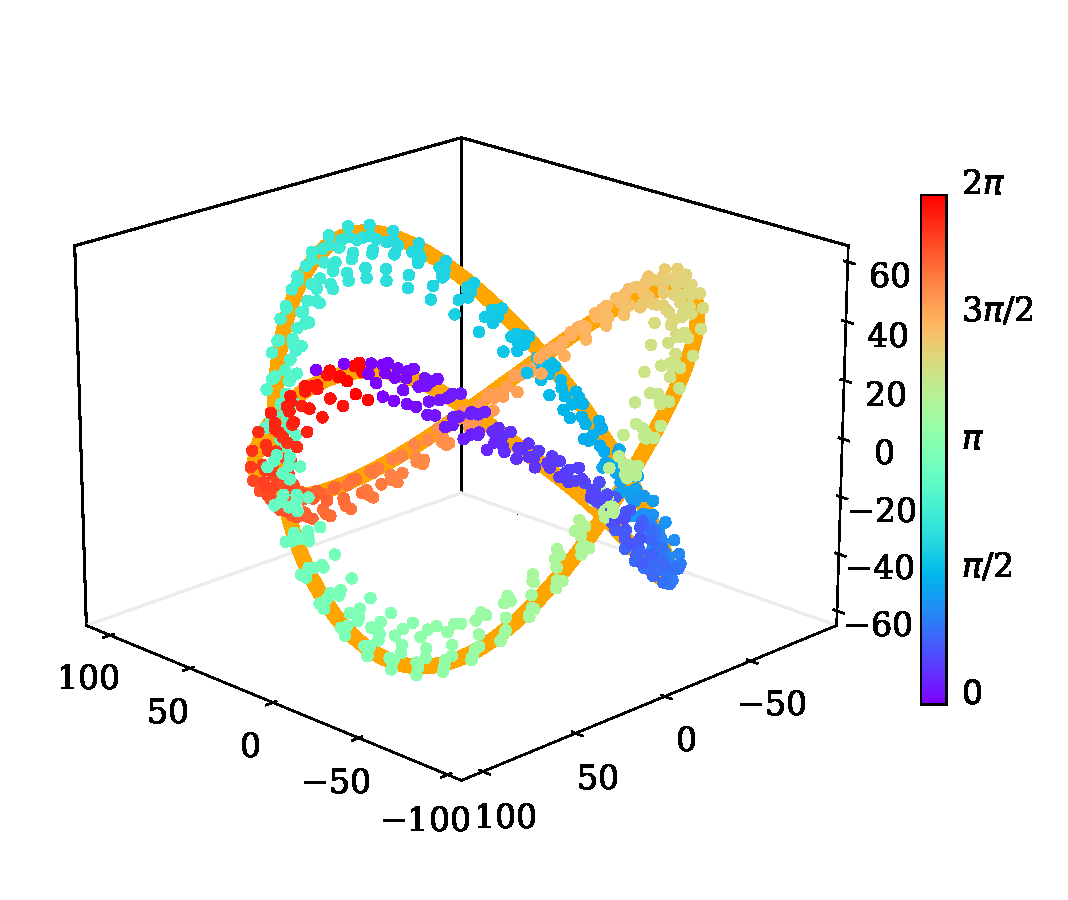
\includegraphics[scale=0.25]{./images/walk_phase.eps} \\ 
            \hline
            
            \rotatebox{90}{ \text{Велопрогулка} }
            & 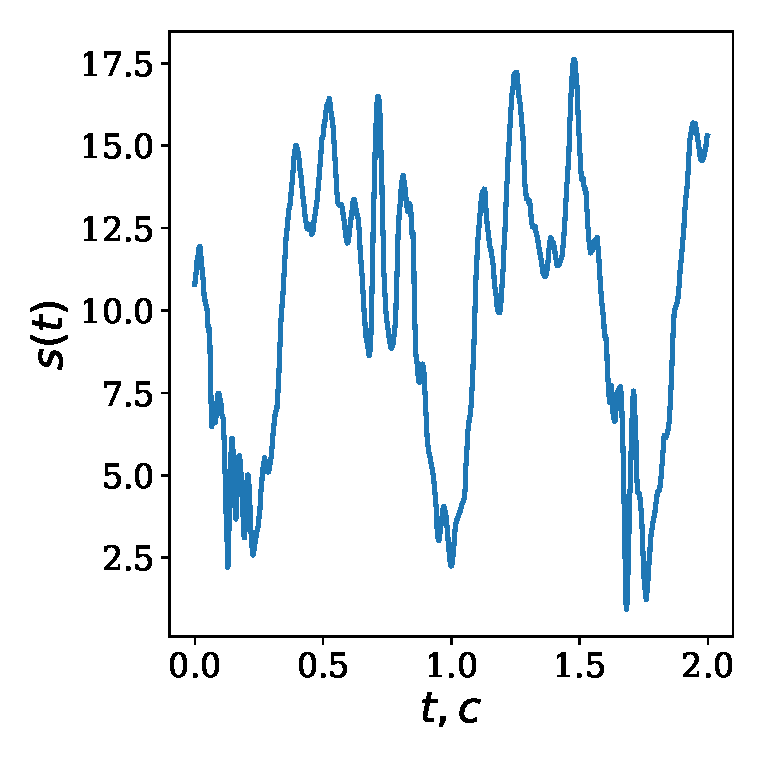
\includegraphics[scale=0.25]{./images/bike_example.eps}
            & 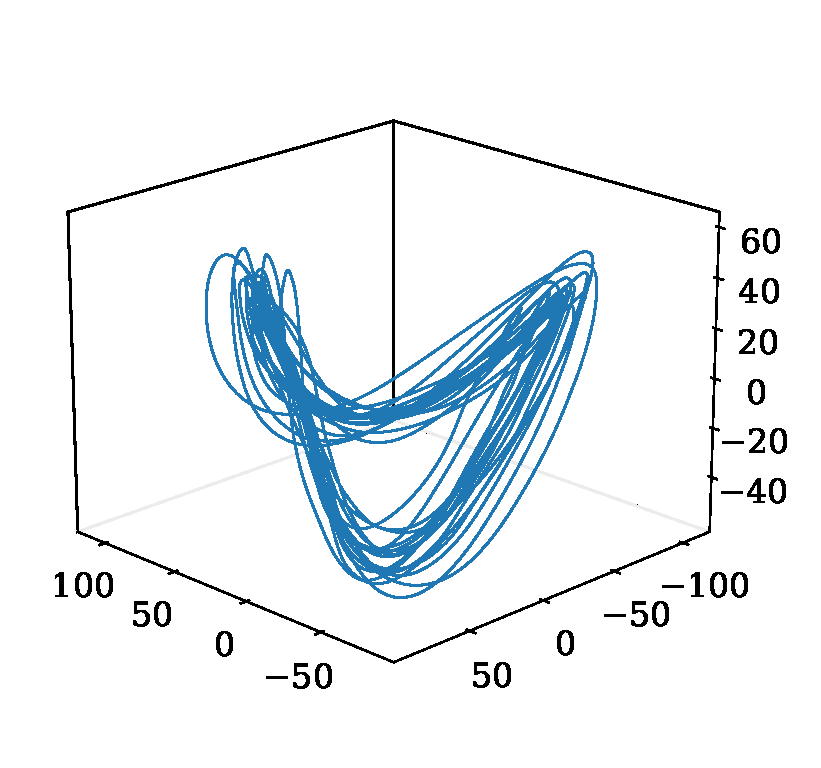
\includegraphics[scale=0.3]{./images/bike_trajectory.eps}
            & 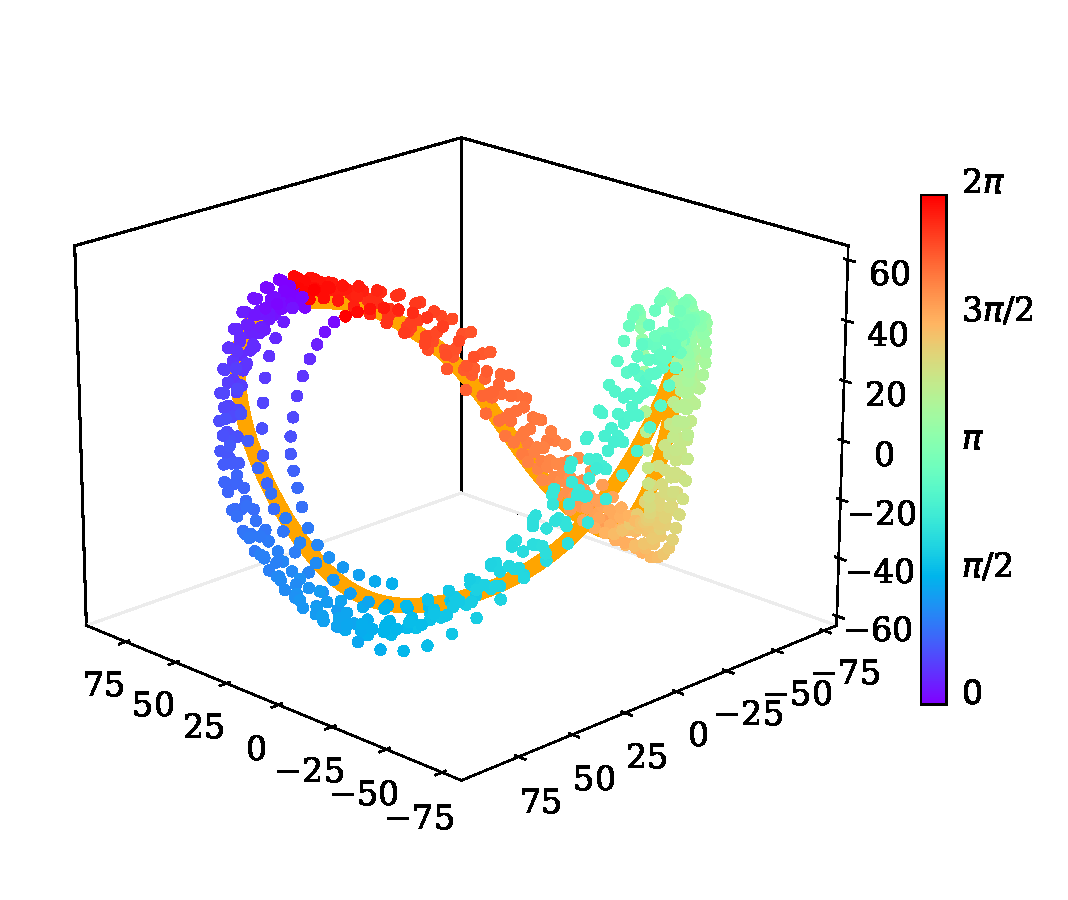
\includegraphics[scale=0.25]{./images/bike_phase.eps} \\ 
            \hline
        
            \bottomrule
        \end{tabular}
    \caption{Результаты работы алгоритма для ходьбы и велопрогулки}
    \label{tbl:table_of_figures}
\end{table}

\end{document}